\documentclass{article}
\usepackage[margin=0.4cm,paperwidth=27cm,paperheight=21cm]{geometry}
\usepackage{amssymb}
\usepackage{tikz}
\usetikzlibrary{arrows.meta,positioning,fit,backgrounds}
\pagestyle{empty}
\begin{document}\centering
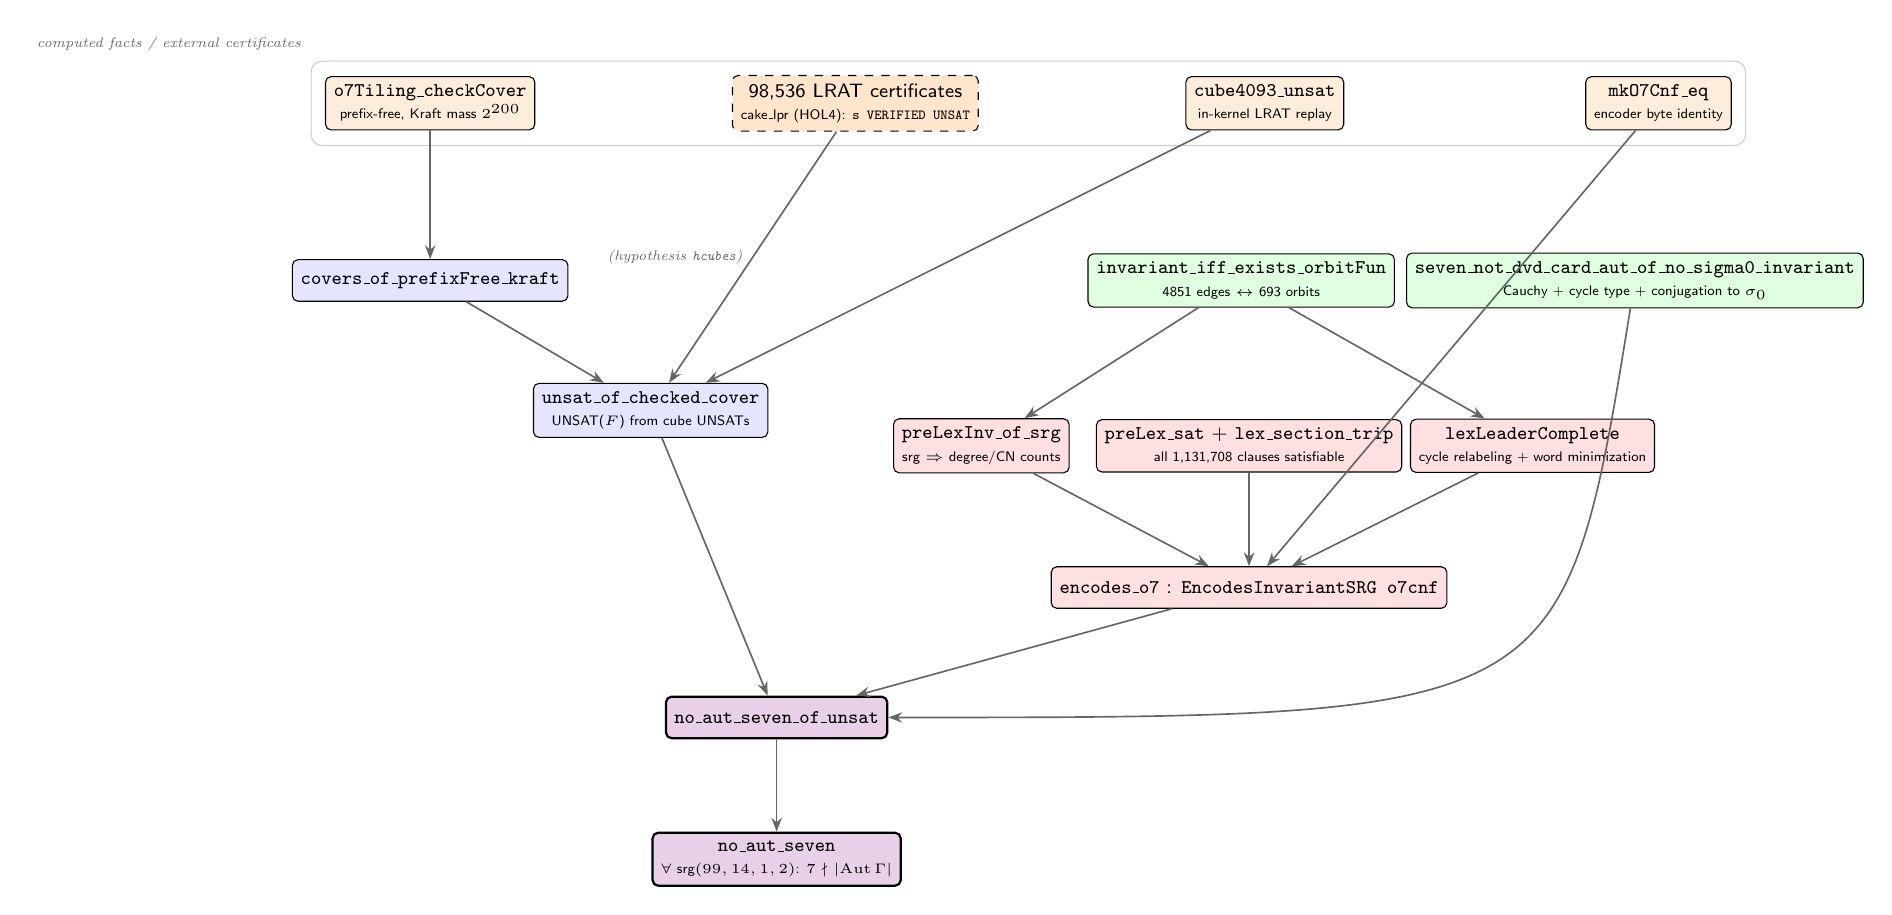
\begin{tikzpicture}[x=1cm,y=1.5cm,
  thm/.style={font=\scriptsize\sffamily,rounded corners=2pt,draw,inner sep=3pt,
              minimum height=15pt,fill=red!8,align=center},
  ext/.style={thm,fill=orange!20,dashed},
  dat/.style={thm,fill=orange!14},
  grp/.style={thm,fill=green!12},
  cov/.style={thm,fill=blue!10},
  enc/.style={thm,fill=red!12},
  fin/.style={thm,fill=violet!18,thick},
  lab/.style={font=\tiny\itshape,text=black!60},
  e/.style={-{Stealth[length=5pt]},semithick,draw=black!60}]

% ---- external / data layer (top) ----
\node[ext] (lrat) at (0,0) {98{,}536 LRAT certificates\\ \tiny cake\_lpr (HOL4): \texttt{s VERIFIED UNSAT}};
\node[dat] (sample) at (5.2,0) {\texttt{cube4093\_unsat}\\ \tiny in-kernel LRAT replay};
\node[dat] (bytes) at (10.2,0) {\texttt{mkO7Cnf\_eq}\\ \tiny encoder byte identity};
\node[dat] (cover) at (-5.4,0) {\texttt{o7Tiling\_checkCover}\\ \tiny prefix-free, Kraft mass $2^{200}$};

% ---- L1 coverage ----
\node[cov] (kraft) at (-5.4,-1.5) {\texttt{covers\_of\_prefixFree\_kraft}};
\node[cov] (unsat) at (-2.6,-2.6) {\texttt{unsat\_of\_checked\_cover}\\ \tiny UNSAT($F$) from cube UNSATs};

% ---- L2/L3 group theory ----
\node[grp] (cyc) at (9.9,-1.5) {\texttt{seven\_not\_dvd\_card\_aut\_of\_no\_sigma0\_invariant}\\ \tiny Cauchy + cycle type + conjugation to $\sigma_0$};
\node[grp] (orb) at (4.9,-1.5) {\texttt{invariant\_iff\_exists\_orbitFun}\\ \tiny 4851 edges $\leftrightarrow$ 693 orbits};

% ---- L4/L5 encoder faithfulness ----
\node[enc] (bridge) at (1.6,-2.9) {\texttt{preLexInv\_of\_srg}\\ \tiny srg $\Rightarrow$ degree/CN counts};
\node[enc] (sections) at (5.0,-2.9) {\texttt{preLex\_sat} + \texttt{lex\_section\_trip}\\ \tiny all 1{,}131{,}708 clauses satisfiable};
\node[enc] (leader) at (8.6,-2.9) {\texttt{lexLeaderComplete}\\ \tiny cycle relabeling + word minimization};
\node[enc] (encodes) at (5.0,-4.1) {\texttt{encodes\_o7} : \texttt{EncodesInvariantSRG o7cnf}};

% ---- endpoints ----
\node[fin] (unsat2) at (-1.0,-5.2) {\texttt{no\_aut\_seven\_of\_unsat}};
\node[fin] (final) at (-1.0,-6.4) {\texttt{no\_aut\_seven}\\ \tiny $\forall$ srg$(99,14,1,2)$: $7 \nmid |\mathrm{Aut}\,\Gamma|$};

\draw[e] (cover) -- (kraft);
\draw[e] (kraft) -- (unsat);
\draw[e] (lrat) -- node[lab,left]{\ (hypothesis \texttt{hcubes})} (unsat);
\draw[e] (sample) -- (unsat);
\draw[e] (orb) -- (bridge);
\draw[e] (orb) -- (leader);
\draw[e] (bytes) -- (encodes);
\draw[e] (bridge) -- (encodes);
\draw[e] (sections) -- (encodes);
\draw[e] (leader) -- (encodes);
\draw[e] (unsat) -- (unsat2);
\draw[e] (encodes) -- (unsat2);
\draw[e] (cyc) .. controls (9,-5.2) .. (unsat2);
\draw[e] (unsat2) -- (final);

\begin{scope}[on background layer]
\node[fit=(cover)(lrat)(sample)(bytes),draw=black!20,rounded corners,inner sep=5pt,
      label={[lab]north west:computed facts / external certificates}] {};
\end{scope}
\end{tikzpicture}
\end{document}
